\documentclass[svgnames]{beamer}
\usetheme{Antibes}

\usepackage{beamerthemesplit}

\usepackage[utf8]{inputenc}
\usepackage[slovene]{babel}
\usecolortheme{beaver}


\title[NROR]{Napredna računalniška orodja - 1. domača naloga}
\author[T. Ulaga]{Tomaž Ulaga}
\institute[FS UL]{Univerza v Ljubljani, Fakulteta za strojništvo}
\date{\today}
\logo{
\includegraphics[width=2.5cm]{fs_ul_logo.png}}



\begin{document}

\frame{\titlepage}

\begin{frame}{Kazalo}
    \tableofcontents
\end{frame}

\AtBeginSection[]{
  \begin{frame}{Kazalo}
    \tableofcontents[currentsection]
  \end{frame}
}

\AtBeginSubsection[]{
  \begin{frame}{Kazalo}
    \tableofcontents[currentsection,currentsubsection]
  \end{frame}
}

\section{Uvod}

\begin{frame}
\frametitle{Uvod}
Domača naloga je zajemala delo s tremi programskimi orodji, to so:
    \begin{itemize}
        \item  Matlab
        \item  GIT
        \item  Beamer (LATEX)
    \end{itemize}
\end{frame}


\section{Matlab}

\begin{frame}
\frametitle{Matlab}

Zahteva naloge je bila: Z uporabo programa Matlab in uporabo metode Monte Carlo za določitev števila \(\pi\).

Ključni koraki so:

    
    \begin{itemize}
        \item Generiranje naključnih števil (oz. koordinat točk)
        \item Definiranje funkcije znotraj funkcijske datoteke
        \item Definiranje anonimne funkcije za določitev krožnice 
        \item Definiranje funkcija za vizualizacijo metode
    \end{itemize}
\end{frame}

\begin{frame}
\frametitle{Matlab}
\begin{figure}
\pi_{prib} =3,1592
    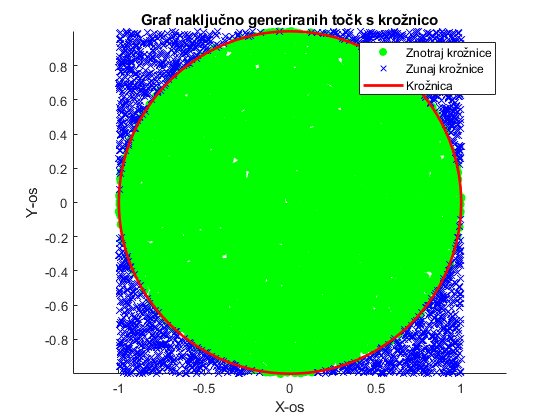
\includegraphics[width=0.7\textwidth]{calc_pi_graf.png}
    \caption{\small Vizualizacija metode Monte Carlo}
\end{figure}
\end{frame}

\section{GIT}
\begin{frame}{GIT}
     \begin{itemize}
        \item Z uporabo orodja Github, smo delili delo s sodelavcem (sošolcem) preko privatnega repozitorija
        \pause
        \item Sodelavec je spremenil datoteko v repozitoriju (Matlab kodo)
        \pause
        \item Kot lastniki repozitorija smo spremembe sprejeli
    \end{itemize}
\end{frame}

\section{BEAMER}
\begin{frame}{BEAMER}
    \begin{itemize}
        \item Pridobljeno znanje programskega jezika Latex, v formatu beamer, smo uporabili za izdelavo te predstavitve
        \item V njej smo na kratko predstavili vsebino 1. domače naloge pri predmetu NROR
        \item Predstavitev vsebuje vse zahteve, podane v navodilih domače naloge
    \end{itemize}
\end{frame}

\end{document}